\documentclass{beamer}
\usetheme{Boadilla}

\usepackage{amsmath}
\usepackage{amsfonts}
\usepackage{hyperref}

\usepackage{amsmath}
\DeclareMathOperator*{\argmax}{arg\,max}
\DeclareMathOperator*{\argmin}{arg\,min}

\newcommand{\bz}{\mathbf{z}}
\newcommand{\bx}{\mathbf{x}}
\newcommand{\by}{\mathbf{y}}
\newcommand{\bv}{\mathbf{v}}
\newcommand{\bw}{\mathbf{w}}
\newcommand{\ba}{\mathbf{a}}
\newcommand{\bb}{\mathbf{b}}
\newcommand{\bff}{\mathbf{f}}
\newcommand{\bh}{\mathbf{h}}
\newcommand{\bl}{\mathbf{l}}
\newcommand{\bp}{\mathbf{p}}
\newcommand{\bq}{\mathbf{q}}
\newcommand{\bs}{\mathbf{s}}
\newcommand{\bt}{\mathbf{t}}
\newcommand{\bu}{\mathbf{u}}
\newcommand{\bT}{\mathbf{T}}
\newcommand{\bX}{\mathbf{X}}
\newcommand{\bZ}{\mathbf{Z}}
\newcommand{\bS}{\mathbf{S}}
\newcommand{\bH}{\mathbf{H}}
\newcommand{\bW}{\mathbf{W}}
\newcommand{\bY}{\mathbf{Y}}
\newcommand{\bU}{\mathbf{U}}
\newcommand{\bQ}{\mathbf{Q}}
\newcommand{\bP}{\mathbf{P}}
\newcommand{\bA}{\mathbf{A}}
\newcommand{\bB}{\mathbf{B}}
\newcommand{\bC}{\mathbf{C}}
\newcommand{\bE}{\mathbf{E}}
\newcommand{\bF}{\mathbf{F}}
\newcommand{\bsigma}{\boldsymbol{\sigma}}
\newcommand{\bomega}{\boldsymbol{\omega}}
\newcommand{\btheta}{\boldsymbol{\theta}}
\newcommand{\bgamma}{\boldsymbol{\gamma}}
\newcommand{\bdelta}{\boldsymbol{\delta}}
\newcommand{\bPsi}{\boldsymbol{\Psi}}
\newcommand{\bpsi}{\boldsymbol{\psi}}
\newcommand{\bxi}{\boldsymbol{\xi}}
\newcommand{\bmu}{\boldsymbol{\mu}}
\newcommand{\bchi}{\boldsymbol{\chi}}
\newcommand{\bzeta}{\boldsymbol{\zeta}}
\newcommand{\blambda}{\boldsymbol{\lambda}}
\newcommand{\beps}{\boldsymbol{\varepsilon}}
\newcommand{\bZeta}{\boldsymbol{Z}}
\newcommand{\dH}{\mathds{H}}
\newcommand{\dR}{\mathds{R}}

\title{Variational Dropout and the Local Reparameterization Trick}
\author{Eduard Vladimirov}
\institute{MIPT, 2023}


\begin{document}

\begin{frame}
    \titlepage
\end{frame}


\begin{frame}
    \tableofcontents
\end{frame}


\section{Motivation \& Background}
\begin{frame}{Motivation}
    \begin{block}{Main idea}
    Efficiency of posterior inference using SGVB can be significantly improved through a local reparameterization.
    
    The authors show how dropout is a special case of SGVB with
    local reparameterization, and suggest variational dropout, an extension of regular
    dropout where optimal dropout rates are inferred from the data.
    \end{block} 
\end{frame}


\begin{frame}{Background}
	\begin{block}{Variational lower-bound}
		\begin{align*}
			\mathcal{L}(\phi) &= -D_{KL}(q_\phi(\bw) || p(\bw)) + L_\mathcal{D}(\phi) \\
			\text{where } L_\mathcal{D}(\phi) &= \sum\limits_{(\bx, \by) \in \mathcal{D}} \mathbb{E}_{q_\psi(\bw)}(\log p(\by | \bx, \bw))
		\end{align*}
	\end{block}
    
    \begin{block}{Stochastic Gradient Variational Bayes}
    \begin{equation*}
        L_\mathcal{D}(\phi) \approx L_\mathcal{D}^{SGVB}(\phi) = \dfrac{N}{M} \sum\limits_{i=1}^M \log p(\by^i | \bx^i, \bw = f(\epsilon, \phi))
    \end{equation*} 

    \begin{enumerate}
	    \item $\nabla_\psi L_\mathcal{D}(\phi) \approx \nabla_\psi L_\mathcal{D}^{SGVB}(\phi)$
    \end{enumerate}
        
    \end{block}
\end{frame}

\section{Theory}
\begin{frame}{Variance of the SGVB estimator}
    \begin{block}{Shorthands}
    	\begin{align*}
    		&L_i := \log p(\by^i | \bx^i, \bw = f(\epsilon, \phi)) \\
    		&L_\mathcal{D}^{SGVB}(\phi) = \dfrac{N}{M} \sum\limits_{i=1}^M L_i \\
    		&Var[L_i] = Var_{\epsilon, \bx^i, \by^i} \bigl[ \log p(\by^i | \bx^i, \bw = f(\epsilon, \phi) \bigr]
    	\end{align*}
    \end{block}

    \begin{block}{Variance}
    	\begin{equation*}
    		Var \bigl[ L_\mathcal{D}^{SGVB}(\phi) \bigr] = N^2 \biggl( \dfrac{1}{M} Var[L_i] + \dfrac{M-1}{M} Cov[L_i, L_j] \biggr)
    	\end{equation*}
    \end{block}
    
\end{frame}


\begin{frame}{Local Reparameterization Trick}
	We want to have $Cov[L_i, L_j] = 0$
	
	Consider simple example: $\bB = \bA \, \bW, \text{ where } \bA, \bB \in \mathbb{R}^{M \times 1000}, \bW \in \mathbb{R}^{1000 \times 1000}$
	
	$q_\phi(w_{i, j}) = \mathcal{N}(\mu_{i, j}, \sigma_{i, j}^2) \; \forall w_{i, j} \in \bW$
	
	$w_{i, j} = \mu_{i, j} + \sigma_{i, j} \epsilon_{i, j}, \text{ with } \epsilon_{i, j} \sim \mathcal{N}(0, 1)$
	
	We have to sample a separate weight matrix $\bW$ for each example in minibatch.
	As a result, we would need to sample M million random numbers for just a single layer!!!
	
\end{frame}

\begin{frame}{Local Reparametrization Trick}
	Solution: sample the random activations $\bB$ directly!
	
	\begin{equation*}
		\begin{split}
			q_\psi(w_{i, j}) &= \mathcal{N}(\mu_{i, j}, \sigma_{i, j}^2) \; \forall w_{i, j} \in \bW \Longrightarrow q_\phi(b_{m, j} | A) = \mathcal{N}(\gamma_{im, j}, \delta_{m, j}), \text{ with} \\
			\gamma_{m, j} &= \sum\limits_{i=1}^{1000} a_{m, i} \mu_{i, j}, \text{ and } \delta_{m, j} = \sum\limits_{i=1}^{1000} a_{m, i}^2 \sigma_{i, j}^2
		\end{split}
	\end{equation*}

	We only need to sample M thousands random variables
	\begin{equation*}
		b_{m,j} = \gamma_{m,j} + \sqrt{\delta_{m,j}} \zeta_{m, j}, \text{ with } \zeta_{m, j} \sim \mathcal{N}(0, 1), \; \zeta \in \mathbb{R}^{M \times 1000}.
	\end{equation*}

	Other advantage: lower variance
\end{frame}

\begin{frame}{Variational Dropout}
	\begin{block}{Dropout}
	    \begin{equation*}
	    	\begin{split}
	    		&\bB = (\bA \circ \xi) \, \theta \quad \text{ with } \xi \sim Bern(1-p), \\ &\text{ where } \bA \in \mathbb{R}^{M \times K}, \theta \in \mathbb{R}^{K \times L}, \bB \in \mathbb{R}^{M \times L},
	    	\end{split}
	    \end{equation*}
	\end{block}
	
	\begin{block}{Gaussian Dropout}
		\begin{equation*}
			\xi \sim \mathcal{N}(1, \alpha), \; \alpha = p / (1-p)
		\end{equation*}
	\end{block}

\end{frame}

\begin{frame}{Variational Dropout}
	\begin{block}{VD with independent weight noise}
		\begin{align*}
			q_\phi(b_{m, j} | A) &= \mathcal{N}(\gamma_{im, j}, \delta_{m, j}) \text{ with } \\
			\gamma_{m, j} &= \sum\limits_{i=1}^{K} a_{m, i} \theta_{i, j}, \text{ and } \delta_{m, j} = \alpha \sum\limits_{i=1}^{K} a_{m, i}^2 \theta_{i, j}^2
		\end{align*}
	\end{block}
	
	\begin{block}{VD with correlated weight noise}
		\begin{align*}
			\bB &= (\bA \circ \xi) \, \theta, \xi_{i, j} \sim \mathcal{N}(1, \alpha) \Longleftrightarrow \bb^m = \ba^m \bW, \text{ with } \\
			\bW &= (\bw_1^`, \ldots, \bw_K^`)^`, \text{ and } \bw_i = s_i \theta_i, \;  q_\phi(s_i) = \mathcal{N}(1, \alpha)
		\end{align*}
	\end{block}
\end{frame}

\section{Empirical results}
\begin{frame}{Variance comparison}
    \begin{figure}[bhtp]
    	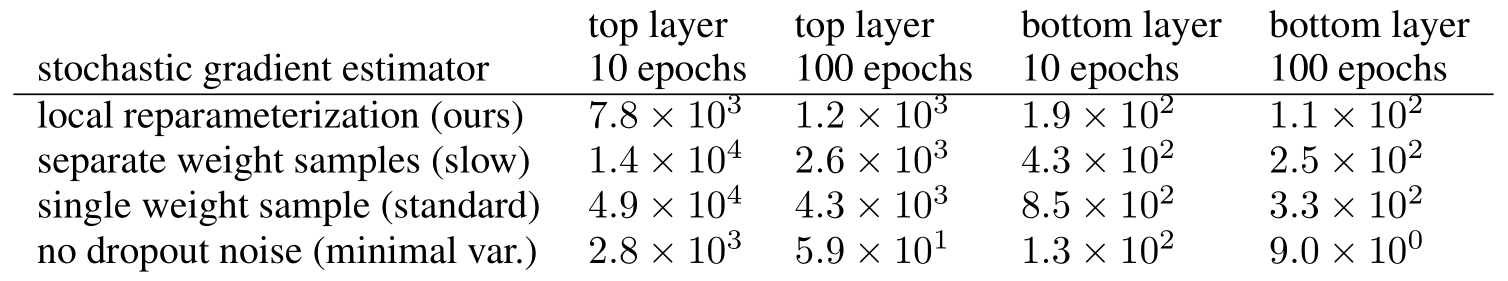
\includegraphics[width=\linewidth]{table.png}
    	\caption{Variance comparison}
    \end{figure}
\end{frame}

\begin{frame}{Different graphics}
	\begin{figure}[bhtp]
		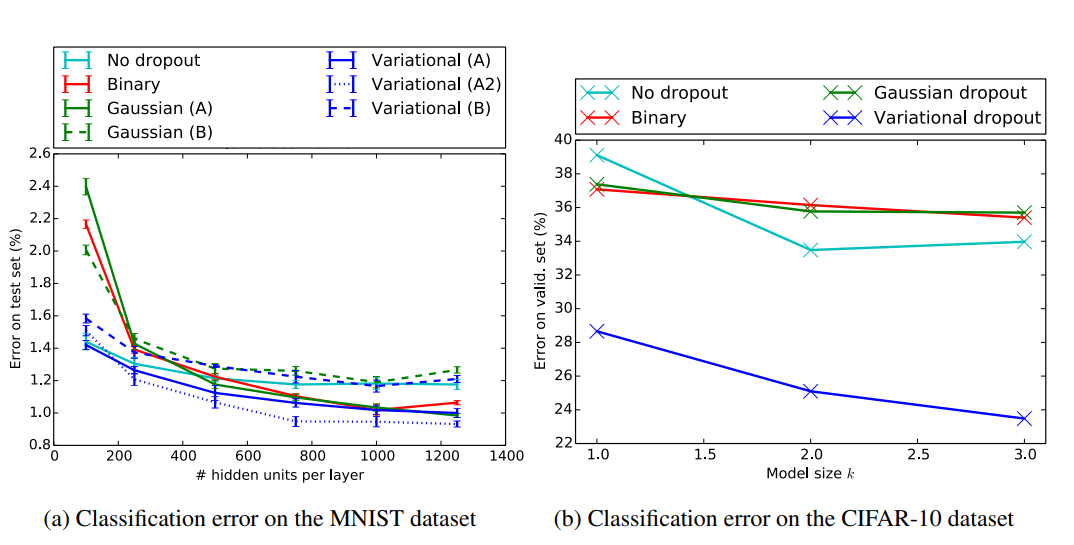
\includegraphics[width=\linewidth]{exp-2.png}
		\caption{Different graphics}
	\end{figure}
\end{frame}


\begin{frame}{Literature}
    \begin{enumerate}
        \item \textbf{Main article} \href{https://arxiv.org/pdf/1506.02557.pdf}
        {Variational Dropout and the Local Reparameterization Trick}.
    \end{enumerate}
\end{frame}



\end{document}